\documentclass[a4paper,10pt]{article}
\usepackage[utf8]{inputenc}
\usepackage[hidelinks]{hyperref}
\def\UrlBreaks{\do\/\do-} % breaks long url in references
\usepackage{graphicx}
\usepackage[english]{babel}
\usepackage{listings}
\usepackage[labelfont=it,
  textfont={it},singlelinecheck=on,justification=centering]{caption}
\usepackage{amsmath}
\usepackage{float}
\usepackage{xcolor}

\lstset{basicstyle=\ttfamily\footnotesize,breaklines=true}
\lstset{numbers=left, numberstyle=\tiny, stepnumber=1, numbersep=5pt}
\lstset{language=TeX}
\setlength{\parskip}{1em}
\renewcommand{\baselinestretch}{1.2}
\newcommand{\x}[1]{{\tt #1}}
\newcommand{\code}[1]{{\tt #1}}
\newcommand{\todo}[1]{{\color{red} TODO #1}}


\title{\textbf{Storj\\A Decentralized Cloud Storage Network Framework}}
\author{\\
\parbox{\linewidth}{\centering\small
Alex Bender (bender@storj.io),
Alex Leitner (alex@storj.io),\\
Benjamin Sirb (bens@storj.io),
Braydon Fuller (braydon@storj.io),\\
Bryan White (bryan@storj.io),
Chris Pollard (cpollard1001@gmail.com),\\
Dennis Coyle (dennis@storj.io),
Dylan Lott (dylan@storj.io),\\
Garrett Ransom (garrett@storj.io),
Gordon Hall (gordonhall@openmailbox.org),\\
James Hagans (jhagans@storj.io),
James Prestwich (james@storj.io),\\
John Gleeson (jg@storj.io),
Josh Brandoff (josh@brandoff.is),
JT Olio (jt@storj.io),\\
Kaloyan Raev (kaloyan@storj.io),
Kishore Aligeti (kishore@storj.io),\\
Nadine Farah (nadine@storj.io),
Natalie Villasana (nat@storj.io),\\
Patrick Gerbes (patrick@storj.io),
Philip Hutchins (philip@storj.io),\\
Shawn Wilkinson (shawn@storj.io),
Tome Boshevski (tome@storj.io)}\\
\\
\small \url{https://github.com/storj/whitepaper}
}
\date {June 24, 2018 \\ v3.0}

\begin{document}
\maketitle

\begin{abstract}
Decentralized cloud storage is attractive for a number of reasons.
Eliminating central control allows users to store and share data without
reliance on a third-party storage provider.
Decentralization mitigates many traditional data failures and outages while it
simultaneously increases security and privacy.
It allows market forces to innovate on cheaper ways to provide storage at a
greater rate than any single entity can afford.
While there are many ways to build such a system, there are some specific
responsibilities any given system should address.
Based on our experience with petabyte-scale storage systems, we introduce a
modular framework for
  considering these responsibilities and building such a system,
  along with initial concrete implementations for each responsibility of the
    framework.
\end{abstract}

\section{Introduction}

Storj is a protocol that creates a distributed network for the reliable storage
of data and facilitates payment for successful data storage between peers. The
Storj protocol enables peers on the network to transfer data, verify the
integrity and availability of remote data, retrieve data, and pay other nodes
for storing data.
Each peer is an autonomous agent, capable of performing these actions without
significant human interaction.

Many storage products have been created based on distributed storage techniques.
Products such as
  Wuala,
  Allmydata,
  Tahoe-LAFS,
  Space Monkey,
  Sia,
  Maidsafe,
  Filecoin,
  Crashplan,
  Mozy,
  HDFS,
  Storj,
  S3,
  GFS,
all share one thing in common: a single computer is not as powerful or as
robust as a network.
These products and others attempt to solve many different use cases and have
many different requirements, but at a high level, they all operate on the same
principles.
They
  generate redundancy for data in case of failure,
  store this redundancy in locations with varying degrees of failure isolation,
  then keep track of where the data was placed.

There are many different primary focuses one could choose when creating a
distributed storage system.
  Speed,
  capacity,
  simplicity,
  trustlessness,
  byzantine fault tolerance,
  security,
  cost,
  etc.,
are all desirable traits in a storage system,
but independently of anything else,
  data must be maintained to prevent data loss,
  nodes in the system must be able to be communicated with,
  and metadata must be kept track of.

While the Storj design space is different from systems such as HDFS or Wuala,
we propose a framework that will allow us to choose some reasonable tradeoffs
and then iterate on improvements to components of the system without changing
the overall system. We accomplish this by breaking the design up into a collection of relatively independent 
concerns, and then bring them together to form the final protocol.

The rest of the paper is divided into 4 sections.
In Section \ref{sec:design_constraints} we discuss the design space Storj operates in and we elaborate on 
some specific design constraints.
Section \ref{sec:framework} covers our framework and proposes a simple concrete implementation of
each framework component.
Section \ref{sec:product_details} covers specific details about how we will ship section \ref{sec:framework} to 
users.
Section \ref{sec:future_work} covers future areas of research.

\section{Storj design constraints and considerations}\label{sec:design_constraints}

Before designing a system, it's important to understand the requirements of
said system, so we'll begin with a discussion of Storj's design constraints.

\subsection{S3 compatibility}

The flagship cloud storage product is Amazon's Simple Storage Service, or S3
for short. Most cloud storage products provide some form of compatibility with
the S3 API.

Until a decentralized cloud storage protocol is the {\em lingua franca} of
storage protocols, a graceful transition must be allowed for users with data
currently on a centralized provider who are interested in the benefits of
decentralized cloud storage but have low tolerance for switching costs.

For Storj to compete successfully in the wider cloud storage industry and bring
decentralized cloud storage to the mainstream -- thus enabling more people
greater security and less centralized control -- applications built against S3
should be able to be made to work with Storj with minimal friction and changes.
This adds strong requirements on feature set, performance, and durability.

\subsection{Byzantine Fault Tolerance}

Unlike datacenter-based solutions like Amazon S3, Storj operates in an
untrusted environment, where individual storage nodes are not necessarily assumed
to be trustworthy. Storj operates over the public internet, and allows
anyone to sign up to become a storage node.

We adopt the BAR (Byzantine, Altruistic, Rational) model \cite{bar} to discuss
participants in the network.
  {\em Byzantine} nodes can depart arbitrarily from a proposed protocol whether it benefits them or not.
  {\em Altruistic} nodes participate in a proposed protocol even if the rational choice is to deviate.
  {\em Rational} nodes participate exactly when it is in their net benefit to do so, and may depart for the same 
reason.

Some distributed storage systems operate in an environment where all nodes are
altruistic {\color{red}add citation?}. Storj operates in an environment where a majority of storage
nodes are rational and a minority are byzantine. Any potential
design must account for this distinction.

\subsection{Device failure and churn}

For any storage system, but especially a distributed storage system, component
failure is a guarantee. All hard drives fail
after enough wear \cite{backblaze-hd-2018-q1}, and the servers providing
the network access to these hard drives will eventually fail, too. Network
links die, power is lost, and storage mediums become unreliable. For data
to outlast individual component failure, data must be stored with enough
redundancy to recover from failure. Perhaps more importantly, no data should be
assumed to be stationary and all data must eventually be moved. In such an environment, redundancy, data 
maintanance, repair, and replacement of lost redundancy are facts of life, and the system must account for 
these issues.

Decentralized systems are additionally susceptible to high churn rates, where potential participants join the 
network and then leave for various reasons, well before their hardware has actually failed. A network with a 
high churn rate will use a large amount of bandwidth just to ensure durability of the data, and such a network 
will fail to scale. As a result, a scalable, highly durable storage system must prefer stable nodes and endeavor 
to keep the churn rate as low as possible. Despite the issues with hardware failure and node churn, 
Maymounkov et al. found that in decentralized systems, the probability of a node staying on for an additional 
hour as a member of the network is an increasing function of uptime \cite{kad}. In other words, the longer a 
node is a participant in the network, the more likely it is to continue participating. See Appendix \todo{} for a 
discussion about how repair bandwidth varies as a function of node churn and uptime.

\subsection{Latency}

Decentralized, distributed storage has massive opportunities for parallelism
with transfer rates, processing, and number of other factors. Parallelism by
itself is a great way to increase overall throughput even when individual
network links are slow. However, parallelism
cannot by itself improve {\em latency}. If an individual network link has fixed
latency and is a required part of an operation, the latency of the overall operation will
be bound from below by the latency of the required network link. Therefore, a distributed system intended for 
high performance applications must aggressively optimize for low latency, both at the individual process scale 
and at the overall architecture scale.

We emphasize an architectural strategy aimed at achieving low latency by focusing on eliminating the need to 
wait for long tails \cite{tail-at-scale}. The goal is a protocol that allows for every request to be satisfiable by the 
fastest nodes participating in any given transaction, without waiting for a slow subset. Focusing on operations 
where the result is only dependent on the fastest nodes
turns what could be a potential liability (highly variable performance from
individual actors) into a great source of strength for a distributed storage
network.

\subsection{Bandwidth}

Global bandwidth availability is increasing year over year, and access
to high-bandwidth internet connections is unevenly distributed. While users in some
countries can easily access symmetric, high-speed, unlimited bandwidth, users in other
countries may have significant difficulty in obtaining access to the same. 
In the United States, many residential internet service providers provide
internet in a way that presents two specific challenges for designers of a decentralized network protocol. 
The first challenge is that the internet connection
is often asymmetric, where customers subscribe to internet service based on the advertised
download speed, and the upload speed is potentially an order of magnitude or
two slower. The second challenge is that bandwidth is sometimes "capped" at a fixed
amount of traffic per month. Such caps impose significant limitations on the bandwidth available at any given 
moment. For example, an internet connection with a throughput of 10 MBPS with a cap of one terabyte per 
month may not average more than 380 KBPS (in a month) without going over the monthly
bandwidth cap.

With device failure and churn guaranteed, any decentralized system will have a corresponding amount of 
repair traffic. It's therefore important to make sure there
is enough headroom for the bandwidth required by data maintenance, over and
above the bandwidth required for data storage and retrieval. 
Designing a storage system that is careless with bandwidth usage would be to
relegate that system below storage providers with access to
unlimited high-speed bandwidth, recentralizing the system to some degree.
To keep the storage system as decentralized as possible and for it to work in as many
environments as possible, bandwidth usage must be aggressively minimized.

Please see Appendix \todo{} for a discussion on how available bandwidth,
combined with required repair traffic, limits usable space.

\subsection{Security and privacy}

\todo{we want to make sure users' data privacy is protected}

\subsection{Object size}

Broadly, large storage systems can be classified into two groups by average
object size. When storing lots of small bits of information, generally a
database is the preferred route. On the other hand, when storing lots of large
files (where "large" files means a few megabytes or more), an object store or
filesystem are ideal.

The initial product offering by Storj Labs is designed to function primarily
as an object store for larger files. While future improvements may enable database-like use cases,
the predominant use case described by this paper is object storage. 
Protocol design decisions are made with the assumption
that the vast majority of objects stored will be a couple of megabytes or more. It is worth pointing out that this 
will not negatively impact use cases that require lots
of files smaller than a megabyte, since such cases can admit a packing strategy, where many small
files are aggregated and stored together as one large file. As the protocol has
streaming support, small files can be retrieved without requiring full
retrieval of any aggregated object they were packed into.

\section{Framework and concrete implementation}\label{sec:framework}

At a high level, there are three major operations in the system: storing data,
retrieving data, and maintaining data.

\begin{description}

\item[Storing data]
When data is stored with the network, the client encrypts it, breaks it up into
multiple little pieces, distributes the pieces to peers in the network, and
generates and stores some metadata about where to find the data again.

\item[Retrieving data]
When data is retrieved from the network, the metadata about where to find the
pieces is recovered first, then the pieces are retrieved and the original data
is reconstructed on the client's local machine.

\item[Maintaining data]
Data is maintained in the network with nodes replacing missing pieces when the amount
of redundancy drops below a certain threshold. The data is reconstructed and the missing pieces are 
regenerated and replaced.

\end{description}

To make this system feasible while satisfying our design constraints, we will
need to solve a number of complex challenges. Inspired by Raft \cite{raft}, we
break the design up into a collection of relatively independent concerns
and then combine them to form the desired protocol. 
One important benefit of doing so is this makes it much easier to
update individual components without rearchitecting the rest of the
network. The individual components are:

\begin{enumerate}
\item Storage nodes
\item Peer-to-peer communication
\item Overlay network
\item Redundancy
\item Structured file storage
\item Metadata
\item Encryption
\item Authorization
\item Data repair
\item Reputation
\item Payments
\end{enumerate}

\subsection{Storage nodes}

The most basic building block is the storage node. The storage node stores and returns data provided to it. Nodes should provide reliable storage space, network bandwidth, and appropriate responsiveness. In return, nodes are rewarded for their participation. Storage nodes will be selected based on a number of different criteria. Ping time, latency, throughput, disk space, geographic location, legal restrictions, etc., are all important factors that may need to be considered.
This means that node selection almost certainly must be an explicit process.

\subsubsection{Concrete implementation}

Storage nodes will support three methods: \code{get}, \code{put}, and
\code{delete}.
Storage nodes store {\em pieces} (to be described in more detail later).
Each method will take
  a {\em piece ID},
  a {\em payer ID} and signature by the payer,
  an optional TTL,
  and the other metadata required by the bandwidth accounting protocol (also
    to be described later).

The \code{put} operation will take a stream of bytes and store the bytes such
that any subrange of bytes can be retrieved again via a \code{get} operation.
\code{get} operations are expected to work until the TTL expires (if a TTL was
provided), or until a \code{delete} operation is received, whichever comes
first.

The {\em payer ID} forms a namespace. An identical {\em piece ID} with a
different {\em payer ID} refers to a different {\em piece}.

Storage nodes should allow administrators to configure maximum allowed disk
space usage and maximum allowed bandwidth usage over the last rolling 30 days.
Storage nodes should keep track of how much is remaining of both. Storage nodes should reject operations that do not have a valid signature from
the appropriate payer.

\subsection{Peer-to-peer communication}

All peers on the network will need to communicate. The framework
requires a reliable and ubiquitous protocol that all peers speak that:

\begin{itemize}
\item provides peer reachability, even in the face of firewalls and NATs. This
 may require techniques like STUN, relays, etc.
\item provides authentication, where each participant knows exactly the
 identity of the peer with whom they are speaking.
\item provides privacy, where only the two peers know what transfers between
 them.
\end{itemize}

\subsubsection{Concrete implementation}

Initially, we'll be using gRPC \cite{grpc} on top of TLS on top of
$\mu$TP \cite{utp} with added STUN functionality. Over time, we'll be
replacing TLS to reduce round trips due to connection handshakes in situations
where the data is already encrypted and forward secrecy isn't necessary.
\todo{} See the Future Work section for more details.

As in S/Kademlia \cite{skad}, the {\em node ID} will be the hash of a
public key and will serve as a proof of work for joining the network. 
Unlike Bitcoin proof of work \cite{bitcoin},
the work will be dependent on how many {\em trailing} zero bits one can find in
the hash output. This means that the node ID will still be usable in a balanced
Kademlia \cite{kad} tree.

The node's master public/private key will only be used to operate a miniature
certificate authority. The node's private key can thus remain in cold storage
if needed. The node will sign keys and certificates to be used for peer-to-peer
communication. When using TLS, every peer can ascertain the ID of the node it
is speaking with by validating the certificate chain and hashing the certificate
authority's key. The peer can estimate how much work went into
constructing that node ID by considering the number of 0 bits at the end of the ID.

For the few cases where a node cannot achieve a successful hole punch through a
NAT or firewall via STUN, uPnP, NATPmP, or a similar technique, manual
intervention and port forwarding will be required.

\subsection{Overlay network}

If, given a peer's network address, any other peer can connect to it, the
framework requires a system to look up peer network addresses by node ID in
the first place. An {\em overlay network} can be built on top of our peer-to-peer communication
component that provides functionality similar to DNS, where a node's ID can be
resolved to an ephemeral network address for communication.

\subsubsection{Concrete implementation}

The Kademlia DHT serves as a key-value store with a built-in node lookup protocol. We utilize this protocol to achieve DNS-like functionality for node lookup, while ignoring the storage aspects of the Kademlia protocol due to some issues around value republishing, limits to network growth rate,
and so on. However, using a DHT will make it difficult to achieve millisecond-level response times when multiple DHT lookups must happen for every operation, so more work is necessary to achieve our performance goals. Fortunately, caching address information for an entire network of 80k nodes (for example) can be done with 3MB of memory, so the DHT can be sped up with some simple, optional
caching.

Because a cache of the DHT can be untrusted (and peer-to-peer
communication is authenticated to avoid man-in-the-middle-attacks anyway),
some well-known community-run DHT caches can be provided that simply attempt to
talk to every storage node every so often, evicting nodes from their cache that
have not been seen recently. Since nodes are expected to be long lived with
good uptime, they are expected to have stable addresses that don't change
often. Thus, such a cache will add a massive performance boost, even when slightly stale. In addition, the protocol will be resilient against an expected degree of node churn, so having a small number of stale addresses in a DHT cache will not alter the expected performance of the network. Furthermore, we avoid a number of known attacks by using the S/Kademlia extensions.

\subsection{Redundancy}

At any moment, any storage node could go offline permanently. Our redundancy
strategy must store data in a way that provides access to the data with high probability, even though any given number of individual nodes may be offline. To achieve a certain level of {\em durability} (the probability that data will remain available in the face of failures), many products in this space use simple replication. Unfortunately, this ties durability to the network {\em expansion factor}, which is the storage overhead for reliably storing data.

As an example, suppose a certain desired level of durability requires a replication strategy that makes eight copies of the data. This yields an expansion factor of 8x, or 800\%. This data then needs to be stored on the network, using bandwidth in the process. Thus, more replication results in more bandwidth usage for a fixed amount of data. As discussed in the protocol design constraints, high bandwidth usage prevents scaling, so this is an undesireable strategy for ensuring a high degree of file durability. Instead, {\em erasure codes} are a more general and more flexible scheme for
manipulating data durability without tying it to bandwidth usage. Importantly, erasure codes allow changes in durability without changes in expansion factor!

An erasure code is often described by two numbers, $k$ and $n$. If a block of
data is encoded with a $(k,n)$ erasure code, there are $n$ total generated
{\em erasure shares}, where only any $k$ of them are required to recover the
original block of data. If a block of data is $s$ bytes, each of the $n$
erasure shares is roughly $s/k$ bytes. Besides the case when $k=1$
(replication), all erasure shares are unique. Interestingly, the durability of a $(k=20,n=40)$ erasure code is better than a $(k=10,n=20)$ erasure code, even though the expansion factor (2x) is the same
for both! Intuitively, this is because the risk is spread across more nodes in
the $(k=20,n=40)$ case. These considerations make erasure codes an important part of our general
framework.

With the simplifying assumption that every node has an equal probability of
failure $p$, one can gain more intuition by modeling file durability as the CDF of the binomial distribution, as seen in Equation \eqref{eq:binom_cdf}. In this case, $P(D)$ represents the probability that at most $n-k$ erasure shares are lost for a given file, so that $n-(n-k)=k$ erasure shares of the file remain; i.e. the file can still be rebuilt.

\begin{equation}
P(D) = \sum_{i=0}^{n-k} \binom{n}{i} p^i (1-p)^{n-i}\label{eq:binom_cdf}
\end{equation}

\begin{table}[b]
	\centering
\begin{tabular}{c c c l}
$k$ & $n$ & Exp. factor & P(D) \\
\hline
2 & 4 & 2 & 99.629999999999996341\%\\
4 & 8 & 2 & 99.956834999999999436\%\\
8 & 16 & 2 & 99.999407567699549748\%\\
16 & 32 & 2 & 99.999999871786737771\%\\
32 & 64 & 2 & 99.999999999999988898\%\\
\end{tabular}
\caption{$P(D)$ for various choices of $k$ and $n$}
\end{table}

\begin{figure}
	\centering
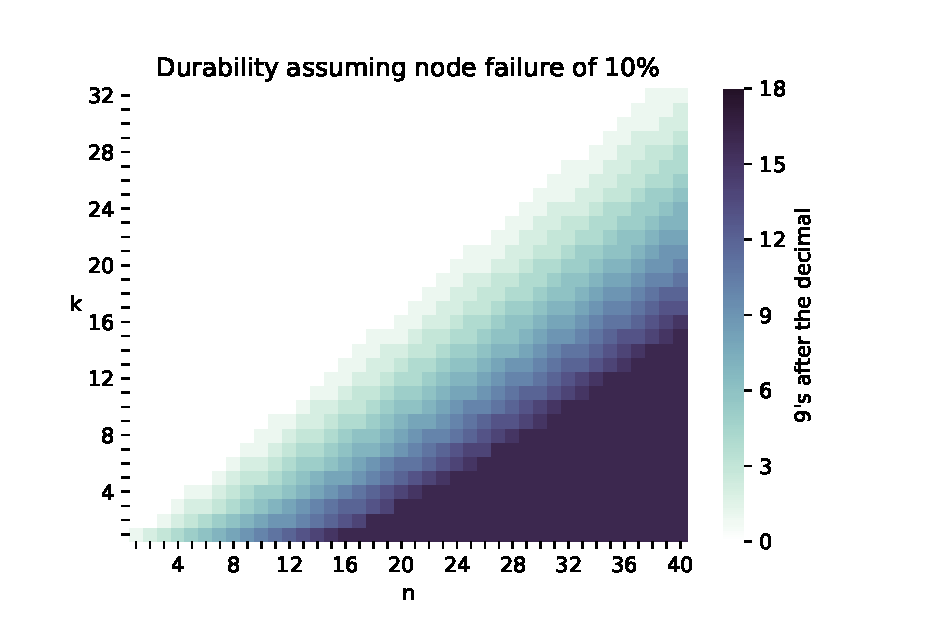
\includegraphics[width=\linewidth]{durability/durability}
\end{figure}


By being able to tweak the durability somewhat independently of the expansion
factor, very high durabilities can be achieved with surprisingly low expansion
factors. Because of how limited bandwidth is as a resource, eliminating
replication as a strategy entirely and using erasure codes only for redundancy
causes a drastic decrease in bandwidth footprint and a drastic increase in the
funds available per byte on storage nodes.

\subsubsection{Streaming}

Erasure codes are used in many streaming contexts such as audio CDs and
satellite communications, so it's important to point out that using
erasure coding in general does not make our streaming design requirement
more challenging. Whatever erasure code is chosen for our framework, streaming
can be added on top by doing encoding in small portions at a time, instead of
attempting to encode a file all at once. See the structured file storage
section for more details.

\subsubsection{Long tails}

Erasure codes enable an enormous performance benefit, which is the ability
to avoid waiting for long-tail response times.\cite{tail-at-scale} For uploads,
a file can be encoded to a higher $(k, n)$ ratio than necessary for durability
guarantees. During an upload, after enough pieces have uploaded to gain
required redundancy, the remaining additional uploads can be canceled, allowing
the upload to only be blocked by the fastest nodes in a set, instead of waiting
for the slowest nodes.

Downloads are similarly improved. Since more redundancy exists than is needed,
downloads can be served from the fastest peers, eliminating a wait for
temporarily slow or offline peers.

\subsubsection{Concrete implementation}

We use the Reed-Solomon erasure code. See \todo{Appendix} for how we selected
our Reed-Solomon numbers.

\subsection{Structured file storage}

Our design constraints include S3 compatibility. This means we should support
hierarchical objects (paths with prefixes), object metadata, arbitrarily large
files, arbitrarily large amounts of files, and so on. Similarly, our design
constraints require security, so any such metadata must be encrypted.

Provided we have an efficient way to store data, we can build many of these
features on top by means of an {\em injective embedding} (here used in the
mathematical sense). Because so many details here depend on concrete
implementation details, our framework is pretty loose in specificity, while
our concrete implementation has significant detail.

\subsubsection{Concrete implementation}

\begin{description}
\item[Bucket] A \x{bucket} is an unbounded but named collection of
\x{file}s identified by \x{path}s. Each \x{path} represents one
\x{file}, and every \x{file} has a unique \x{path}.

\item[Path] A \x{path} is a unique identifier for a \x{file} within a
\x{bucket}. A \x{path} is a string of UTF8 codepoints that begins with a forward
slash and ends with something besides a forward slash. More than one forward
slash (referred to as the \x{path separator}) separate \x{path components}.

An example path might be \code{/etc/hosts}, where the \x{path components} are
\code{etc} and \code{hosts}.

Clients encrypt \x{paths} before they ever leave the client computer.

\item[File] A \x{file} is a collection of \x{stream}s. Every \x{file} has
exactly one default \x{stream} and may have 0 or more named \x{stream}s.
Multiple \x{stream}s allow flexible support of extended attributes, alternate
data streams, resource forks, and other slightly more esoteric filesystem
features.

Like \x{path}s, the data contained in a \x{file} is encrypted before it ever
leaves the client computer.

\item[Stream] A \x{stream} is an ordered collection of 0 or more \x{segment}s.
\x{segment}s have a fixed maximum size, and so the more bytes the \x{stream}
represents through \x{segment}s, the more \x{segment}s there are.

\item[Segment] A \x{segment} represents a single array of bytes, between 0 and a
user-configurable maximum \x{segment} size. Breaking large \x{file}s into
multiple \x{segment}s provides a number of security and scalability advantages.

\item[Inline Segment] An \x{inline segment} is a \x{segment} that is small
enough it makes sense to store it "inline" with the metadata that keeps track of
it, such as a \x{pointer}.

\item[Remote Segment] A \x{remote segment} is a larger \x{segment} that will be
encoded and distributed across the network. A \x{remote segment} is larger than
the metadata required to keep track of its book keeping.

\item[Stripe] A \x{stripe} is a further subdivision of a \x{segment}. A \x{stripe}
is a fixed amount of bytes that is used as an encryption and erasure encoding
boundary size. Encryption and erasure encoding happen on \x{stripe}s
individually. Encryption happens on all \x{segment}s, but erasure encoding only
happens on \x{remote segment}s.

\item[Erasure Share] When a \x{segment} is a \x{remote segment}, its \x{stripe}s
will get erasure encoded. When a \x{stripe} is erasure encoded, it generates
multiple pieces called \x{erasure share}s. Only a subset of the
\x{erasure share}s are needed to recover the original \x{stripe}, but each
\x{erasure share} has an index identifying which \x{erasure share} it is (e.g.,
the first, the second, etc.).

\item[Piece] When a \x{remote segment}'s \x{stripe}s are erasure encoded into
\x{erasure share}s, the \x{erasure share}s for that \x{remote segment} with the
same index are concatenated together, and that concatenated group of
\x{erasure share}s is called a \x{piece}. If there are $n$ \x{erasure share}s
after erasure encoding a \x{stripe}, there are $n$ \x{piece}s after processing
a \x{remote segment}. The $i$th \x{piece} is the concatenation of all of the
$i$th \x{erasure shares} from that \x{segment}'s \x{stripe}s.

\item[Piece Storage Node] A node in the network that is responsible for storing
\x{piece}s. These are operated by \x{farmer}s.

\item[Farmer] A person or group that is responsible for running and maintaining
\x{piece storage nodes}.

\item[Pointer] A \x{pointer} is a data structure that keeps track of which
\x{piece storage nodes} a \x{remote segment} was stored on, or the
\x{inline segment} data directly if applicable.

\end{description}

\subsubsection{Files as Streams}

Many applications benefit from being able to keep metadata alongside files.
For example, NTFS supports "alternate data streams" for each file, HFS supports
resource forks, EXT4 supports "extended attributes," and more importantly for
our purposes, AWS S3 supports "object metadata."\cite{s3-object-meta} Being
able to support arbitrarily named sets of keys/values dramatically improves
compatibility with other storage platforms.

Every \x{file} will have at least one \x{stream} (the default \x{stream}) and
many files may never have another \x{stream}.

\subsubsection{Streams as Segments}

Because \x{stream}s are used for data (the default \x{stream}) and metadata
(extended attributes, etc.), \x{stream}s should be designed both for small data
and large data. If a \x{stream} only has very little data, it will have one
small \x{segment}. If that \x{segment} is smaller than the metadata it would
require to store across the network, the \x{segment} will be an
\x{inline segment} and the data will be stored directly inline with the
metadata.

For larger \x{stream}s, past a certain size the data will be broken into
multiple large \x{remote segment}s. Segmenting in this manner has a number of
advantages to security, privacy, performance, and availability.

Maximum \x{segment} size is a configurable parameter. To preserve privacy, it is
recommended that \x{segment} sizes be standardized as a byte multiple, such as 8
or 32 MB. Smaller \x{segment}s may be padded with zeroes or random data.
Standardized sizes help frustrate attempts to determine the content of a given
\x{segment} and can help obscure the flow of data through the network.

Segmenting large files like video content and distributing the \x{segment}s
across the network separately reduces the impact of content delivery on any
given node.
Bandwidth demands are distributed more evenly across the network. In addition,
the end-user can take advantage of parallel transfer, similar to
BitTorrent\cite{24} or other peer-to-peer networks.

\subsubsection{Segments as Stripes}

In many situations it's important to be able to access just a portion of some
data. Some large file formats such as large video files, disk images, or file
archives support the concept of seeking, where only a partial subset of the
data is needed for correct operation. In these cases it's useful to be able to
decode and decrypt only parts of a file.

A \x{stripe} is no more than a couple of kilobytes, and encrypting and encoding
a single \x{stripe} at a time allows us to read portions of a large \x{segment}
without retrieving the entire \x{segment}, allows us to stream data into the
network without staging it beforehand, and enables a number of other useful
features.

\x{stripe}s should be encrypted client-side before being erasure encoded. The
reference implementation uses AES256-GCM by default but XSalsa20+Poly1305 is
also provided. This protects the content of the data from the \x{farmer} housing
the data. The data owner retains complete control over the encryption key, and
thus over access to the data.

It's important to use authenticated encryption to defend against data
corruption (willful or negligent), and with a monotonically increasing
nonce to defeat reordering attacks. The nonce should be monotonically increasing
across \x{segment}s throughout the \x{stream}. If \x{stripe} $i$ is encrypted
with nonce $j$, \x{stripe} $i+1$ should be encrypted with nonce $j+1$. Each
\x{segment} should get a new encryption key whenever the content in the
\x{segment} changes to avoid nonce reuse.

\subsubsection{Stripes as Erasure Shares}

Erasure encoding gives us the chance to control network durability in the face
of unreliable \x{piece storage node}s. Erasure encoding schemes often are
described as $(n, k)$ schemes, where $k$ \x{erasure shares} are needed for
reconstruction out of $n$ total. For every \x{stripe}, $n$ \x{erasure share}s
are generated, where the network has an expansion factor of $\frac{n}{k}$.

For example, let's say a \x{stripe} is broken into 40 \x{erasure share}s
($n=40$), where any 20 ($k=20$) are needed to reconstruct the \x{stripe}. Each
of the 40 \x{erasure share}s will be $\frac{1}{20}$th the size of the original
\x{stripe}.

All $n$ \x{erasure share}s have a well defined index associated with them. The
$i$th share will always be the same, given the same input parameters.

Because peers generally rely on separate hardware and infrastructure, data
failure is not correlated. This implies that erasure codes are an extremely
effective method of securing availability. Availability is proportional to the
number of nodes storing the data.

See section \todo{} for a breakdown of how varying the erasure code parameters
affects availability and redundancy.

\subsubsection{Erasure Shares as Pieces}

Because \x{stripe}s are already small, \x{erasure share}s are often
much smaller, and the metadata to keep track of all of them separately would be
immense relative to their size. Instead of keeping track of all of the shares
separately, we pack all of the \x{erasure share}s together into a few
\x{piece}s. In an $(n, k)$ scheme, there are $n$ \x{piece}s, where each
\x{piece} $i$ is the ordered concatenation of all of the \x{erasure share}s
with index $i$.

As a result, where each \x{erasure share} is an $\frac{n}{k}$th of a \x{stripe},
each \x{piece} is an $\frac{n}{k}$th of a \x{segment}, and only $k$ \x{piece}s
are needed to recover the full \x{segment}.

\subsubsection{Pointers}

\todo{}

\subsection{Metadata}

In the previous section, we discussed how we will break up files,
encode them for redundancy, and then store them in the network. Independently
of the concrete organization and structure of this scheme, there are two
types of metadata that are important to store somewhere for recovery:
paths and what storage nodes received pieces (pointers).

Our framework requires a relatively performant system that can store
pointers by path in a way that supports ordered iteration over those paths.
Every time an object is added, edited, or removed, one or more entries in this
metadata storage system will need to be adjusted. As a result, there could be
heavy churn in this metadata system, and across the entire
userbase the metadata itself could end up being a sizeable amount of data.

To talk more about the scope and scale we expect with some examples,
suppose in a few years this system stores 1 total exabyte of data,
where the average object size is 50MB and our erasure code is such that $n=40$.
Each object will use just one segment, and thus have one pointer each. The
pointer will contain information about the segment encoding, including what
$n$ nodes the segment pieces are stored on. 1 exabyte of 50MB objects is still
20 billion objects. If each pointer is roughly 40*64+192 bytes (info for each
node plus the path and some general overhead), there are over 55 terabytes of
metadata to keep track of (which is still 18,181 times less data to keep track
of than an exabyte). Fortunately, this metadata can be heavily partitioned by
user. A user storing a 100 terabytes of 50MB objects will only incur an
overhead of 5.5 gigabytes, once again 18,181 times less data. It's worth
pointing out that these numbers vary heavily with average object size (the
larger the object size, the less the metadata overhead).

Otherwise, aside from scale requirements, the desired API is straightforward
and simple: Put (store a pointer given a path), Get (retrieve a pointer given a
path), List (paginated, ordered listing of existing paths), and Delete (remove a
path).

One of our framework's primary focuses is making sure this component, metadata
storage, is interchangeable per user. Specifically, we expect to ship with
multiple implementations of metadata storage that we will allow users to choose
between. Other systems have spent an enormous amount of time attempting to
solve this problem. We've concluded that multiple {\em good enough} solutions
already exist, and propose using them.

\subsubsection{Aside about distributed consensus}

Getting a group of computers to agree on a set of values, and thus constructing
a horizontally-scalable database that works in the face of even just
crash failures (failures where a server simply shuts down), has
been a long and challenging area of research. Fortunately, it has ultimately
led to some really exciting technology.

The biggest issue with getting a group of computers to agree is that messages
can be lost. How this impacts decision making is succinctly
described by the "Two Generals' Problem"\cite{two-generals} (earlier described
as a problem between groups of gangsters\cite{two-gangsters}), in which two
armies try to communicate in the face of potentially lost messages. Both armies
have already agreed to attack a shared enemy, but have yet to decide on a time.
Both armies must attack at the same time or else failure is assured.
Both armies can send messengers, but the messengers are often captured by the
enemy.
Both armies must know what time to attack and that the other army has also
agreed to this time.

Ultimately a solution to the two generals' problem with a finite number of
messages has been proven to be impossible, so engineering approaches have by
necessity had to brace uncertainty.
Many distributed systems make trade-offs to deal with this uncertainty. Some
systems embrace {\em consistency}, which means that the system will choose
downtime instead of inconsistent answers. Other systems embrace
{\em availability}, which means that the system chooses potentially inconsistent
answers instead of downtime. The widely-cited CAP theorem\cite{cap} states that
every system must choose only two of consistency, availability, and partition
tolerance. Due to the inevitability of network failures, partition tolerance
is non-negotiable, and when a partition happens, every system must choose
to sacrifice either consistency or availability. Note that many systems
(sometimes by accident) sacrifice both.

In the CAP theorem, consistency means that every read receives the most recent
write or an error, so an inconsistent answer means the system returned something
besides the most recent write without obviously failing. More generally, there
are a number of {\em consistency models} that may be acceptable by making
various tradeoffs. Linearizability, sequential consistency,
causal consistency, PRAM consistency, eventual consistency, read-after-write
consistency, etc., are all models for discussing how a history of events appears
to various participants in a distributed system.\footnote{If
differing consistency models are new to you, it may be worth reading about them
in Kyle Kingbury's excellent tutorial\cite{aphyr-consistency}.
If you're wondering why computers can't just use the current time to
order events, keep in mind it is exceedingly difficult to get computers to even
agree on that\cite{no-now}.}

Amazon S3 in general provides {\em read-after-write consistency}, though in
some cases will provide {\em eventual consistency} instead\cite{s3-consistency}.
Arguably, there may be some flexibility here for the selection of alternate
consistency models that suit us better while still broadly providing S3
compatibility. Many distributed databases provide eventual consistency by
default, such as Dynamo\cite{dynamo} and Cassandra\cite{cassandra}.

Linearizability in a distributed system is often much more desirable, as it
is useful as a building block for many higher level data structures and
operations such as distributed locks and other coordination techniques.
Initially, early efforts centered around two-phase commit, then three-phase
commit, which both suffered due to issues similar to the two generals' problem.
Things were looking bad in 1985 when the FLP-impossibility paper\cite{flp}
proved that no algorithm could reach linearizable consensus in bounded time.
Then in 1988, Barbara Liskov and Brian Oki published the Viewstamped Replication
algorithm\cite{vr} which was the first linearizable distributed consensus
algorithm. Unaware of the VR publication, Leslie Lamport set out to
prove linearizable distributed consensus was impossible\cite{paxos-note}, but
instead in 1989 proved it was possible by publishing his own Paxos
algorithm\cite{paxos}, which for some reason became significantly more popular.
Ultimately both algorithms share a significant degree of commonality.

Despite Lamport's claims that Paxos is actually simple in his paper
Paxos Made Simple\cite{paxos-simple}, many papers have been published since
then challenging that assertion. Google's description of their attempts to
implement Paxos landed in Paxos Made Live\cite{paxos-live}, Paxos Made
Moderately Complex\cite{paxos-complex} is an attempt to try and fill in all the
details of the protocol, and the entire basis of the Raft algorithm is rooted
in trying to wrangle and simplify the complexity of Paxos\cite{raft}.
Ultimately, to summarize the situation briefly, after an upsetting few decades,
reliable implementations of Paxos, Raft, Viewstamped Replication\cite{vrr},
Chain Replication\cite{chain-rep}, and Zab\cite{zab} now exist, with ongoing
work to improve the situation further\cite{epaxos}\cite{paxos-flexible}.

Arguably, part of Google's early success was in spending the time to build
their internal Paxos-as-a-service distributed lock system, Chubby\cite{chubby}.
Most of Google's most famous internal data storage tools such as
Bigtable\cite{bigtable} depend on Chubby for correctness.
Spanner\cite{spanner}, perhaps one of the most incredible distributed databases
in the world, is mainly just two-phase commit on top of multiple Paxos groups.

Reliable distributed consensus algorithms have been game changing for
many applications needing fault-tolerant storage.

\subsubsection{Aside about Byzantine distributed consensus}

As mentioned in our design constraints, we expect most nodes to be
{\em rational} and some to be {\em byzantine}, but few-to-none to be
{\em altruistic}. Unfortunately, all of the previous algorithms we discussed
assume a collection of altruistic nodes.

There have been a number of attempts to solve the Byzantine fault
tolerant distributed consensus problem (PBFT\cite{pbft} (Barbara Liskov again
with the first solution out of the gate), Q/U\cite{qu},
FaB\cite{fab} (but see \cite{fab-revisited}), Bitcoin\cite{bitcoin},
Zyzzyva\cite{zyzzyva} (but also see \cite{fab-revisited}),
RBFT\cite{rbft}, Tangaroa\cite{tangaroa}, Tendermint\cite{tendermint},
Aliph\cite{aliph}, Hashgraph\cite{hashgraph}, HoneybadgerBFT\cite{honeybadger},
Algorand\cite{algorand}, Casper\cite{casper}, Tangle\cite{tangle},
Avalanche\cite{avalanche}, PARSEC\cite{parsec}, and others\cite{mickens-bft}).

Each of these algorithms make some additional tradeoffs the non-Byzantine
distributed consensus algorithms don't need to make to deal with the potential
for uncooperative nodes. For example, PBFT causes a significant amount of
network overhead. Bitcoin intentially limits the transaction rate with
changing proof-of-work difficulty, in addition to, like other blockchain-based
solutions, requiring all participants to keep a full copy of all change
histories.

\todo{talk about merkle-dag, git-inspired approaches to metadata, potentially
built on kademlia, potentially reworking this entire section because ugh}

\subsubsection{Concrete implementation}

Given the situation described in the asides about distributed consensus, we
have decided that--for our initial release--good enough solutions already exist,
so we will punt the problem of solving Byzantine distributed consensus for
our use case to a later release. We believe that a great distributed algorithm
here is possible, all of the necessary building blocks are likely described
above, and expect to invest heavily in research to find it after we have a
thriving user base with our solution based on good enough approaches.

The most trivial implementation for the metadata storage functionality we
require would be to simply have each user use their preferred trusted database
such as PostgreSQL, SQLite, MongoDB, Cassandra\cite{cassandra},
Spanner\cite{spanner}, CockroachDB, or something else. In many cases, this will
be acceptable for specific users, provided those users were managing
appropriate backups of their metadata. Indeed, the types of users who have
petabytes of data to store probably can manage reliable backups of a single
relational database storing only metadata.

There are a few downsides with this punt-to-the-user approach, however, such as:
\begin{itemize}
\item {\bf Availability} - the availability of the user's data is tied entirely
  to the availability of their metadata server. The counterpoint here is that
  the availability can be made arbitrarily good with existing trusted
  distributed solutions such as Cassandra, Spanner, or CockroachDB. Further,
  any individual metadata service downtime does not affect the entire network.
  In fact, the network as a whole can still never go down.
\item {\bf Durability} - if the metadata server suffers a catastrophic failure
  without backups, all of the user's data is gone. This is already true with
  encryption keys, but a punt-to-the-user solution increases the risk area from
  just encryption keys considerably. Fortunately, the metadata itself can be
  periodically backed up into the Storj system, such that only needing
  to keep track of metadata-metadata further decreases the amount of critical
  information that must be stored elsewhere.
\item {\bf Trust} - the user has to trust the metadata server.
\end{itemize}

On the other hand, there are a few upsides:
\begin{itemize}
\item {\bf Use cases} - in a catastrophic scenario, this design still covers
  all required use cases.
\item {\bf Control} - the user is in complete control of all of their data.
  There is still no organizational single point of failure. The user is free
  to choose whatever metadata store with whatever tradeoffs they like.
  Like Mastodon\cite{mastodon}, this solution is still decentralized.
  Further, in a catastrophic scenario, this design is no worse than most other
  technologies or techniques application developers frequently use (databases).
\item {\bf Simplicity} - other projects have spent multiple years on shaky
  implementations. We can get a useful product to market without doing this
  work at all. This is a considerable advantage.
\end{itemize}

Our launch goal is to allow customers to store their metadata in a database
of their choosing. We expect and look forward to new systems and improvements
specifically in this component of our framework.

\subsection{Encryption}

\subsubsection{Concrete implementation}

\subsection{Authorization}

\subsubsection{Concrete implementation}

\subsection{Data repair}

\todo{thresholds}
\todo{
To prevent loss of the file, data owners should set shard loss tolerance levels.
Consider a 20-of-40 erasure coding scheme. A data owner might tolerate the loss
of 5 shards out of 40, knowing that the chance of 16 more becoming inaccessible
in the near future is low. However, at some point the probabilistic availability
will fall below safety thresholds. At that point the data owner must initiate a
retrieve and rebuild process.

Because node uptimes are known via the audit process, tolerance levels may be
optimized based on the characteristics of the nodes involved. Many strategies
may be implemented to handle this process.
}

\subsubsection{Concrete implementation}

\subsection{Reputation}

\subsubsection{Concrete implementation}

\subsection{Payments}

\subsubsection{Concrete implementation}

\subsection{Encryption}

\todo{}

\subsection{Structured file storage}

\subsection{Network state}
Overview
The network state is a component of the distributed network, and has a primary
role of storing information related to the segment. The network state keeps
track of \x{pointer}s, which contain the IDs of \x{piece storage nodes} holding \x{remote
segment}s, indication if the segment is \x{inline} and other descriptors. The network
state service houses a \x{pointer} database that can be called by other services
to put, get, list, and delete \x{pointers}.

Two components of the distributed network depends on the network state: the light
client and repair and maintenance (also known as data repair). The light client
makes requests to the network state to store or receive \x{pointer}s to \x{segment}s
depending on if there is an upload or download action. Similarly, the data repair
will request and receive a list of \x{pointer}s. Each \x{pointer} contains the metadata
mentioned above including the following values related to Reed Solomon encoding: the
minimum number of \x{piece}s required for a \x{segment}'s reconstruction, the total
amount of \x{pieces} generated through erasure encoding, the repair threshold, or
number of pieces needed to lose before triggering repair, and the success threshold,
or amount of pieces needed to be stored in order to be counted as a success. Below
are descriptions of how the light client and data repair interact with the network
state for uploads, downloads, and data repair, respectively.


\subsubsection{Download General Overview}
In order to download a file, the light client will login and send a request to the
network state to get pointers to the stored segments, and other metadata. The light
client extracts the node IDs that are storing the data and send a request to the overlay
network with those IDs. The overlay network responds with an object containing the nodes’
IP addresses. Finally, the light client sends a request to farmers in order to receive
pieces using those IP addresses.


Technical Dive into how Download Works
\todo{}

Upload General Overview
In order to upload a file, the light client will log in and ask the overlay network
for a set of farmers that fulfill a criteria, i.e. storage availability and bandwidth
to potentially store files. The overlay network will have a list of nodes that meet
those criteria and use the reputation network to filter out reputable farmers. The
overlay network then sends a refined list of farmers to the light client, which is
then used to directly upload data. Finally, the light client sends a request to the
network state in order to store the IDs of the piece storage nodes holding the segments
and other related metadata in pointers.


Technical Dive into how Upload Works
\todo{}

Repair and Maintenance
The repair and maintenance component (also known as data repair) is essential to ensure
data integrity is maintained. It confirms that nodes responsible for pieces continue to
store the data that the light client sent. To do this, it first makes a request to the
network state to receive pointers. From there, the repair and maintenance component
extracts the node IDs from the response and makes a request with that information to the
DHT cache. The DHT cache sends a response containing only the online nodes from the original
node ID list. The data repair component takes the response from the DHT cache and the
repair threshold value from the pointer, then calculates which pieces need to get repaired. The
light client directly downloads pieces that need to get repaired from farmers and re-uploads
them to new reputable farmers. To ensure the network state has up-to-date information about
the data, the light client then sends a put request of new pointers with the updated node IDs.


Diagram Technical Detail
<WIP>

\subsection{Authorization}

\todo{}

\subsection{Farmer Reputation}

\todo{}

\subsection{Payments}

\todo{}

\subsection{Payer Reputation}

\todo{}

\subsection{Repair and Maintenance}

\todo{discussion about audits using erasure codes instead of challenge merkle trees}
\todo{discussion about spot checks}

\todo{

Partial audits provide only probabilistic assurance that the farmer retains the
entire file. They allow for false positive results, where the verifier believes
the farmer retains the intact shard, when it has actually been modified or
partially deleted. The probability of a false positive on an individual partial
audit is easily calculable (see Section 6.4)

Thus the data owner can have a known confidence level that a shard is still
intact and available. In practice, this is more complex, as farmers may
implement intelligent strategies to attempt to defeat partial audits.
Fortunately, this is a bounded problem in the case of iterative audits. The
probability of several consecutive false positives becomes very low, even when
small portions of the file have been deleted.
}

\subsection{Payment}

\todo{
Storj is payment agnostic. Neither the protocol nor the contract requires a
specific payment system. The current implementation assumes Storjcoin, but many
other payment types could be implemented, including BTC, Ether, ACH transfer, or
physical transfer of live goats.
}

\section{Product details}\label{sec:product_details}

\todo{
The client provides the actual storage API. It should be run co-located with
wherever data is generated, and will communicate directly with storage nodes
so as to avoid central bandwidth costs. The client can provide an S3-compatible
API to interoperate with existing software.

When data is sent to the client, the client will encrypt the data, choose
appropriate storage nodes, store the data on those nodes, then use the metadata
system to keep track of which nodes the data resides on for future reading.
}

\subsection{Farmer}

\todo{}

\subsection{Bridge}

\todo{
As should be apparent, the data owner has to shoulder significant burdens to
maintain availability and integrity of data on the Storj network. Because nodes
cannot be trusted, and hidden information like challenge sets cannot be safely
outsourced to an untrusted peer, data owners are responsible for negotiating
contracts, pre-processing shards, issuing and verifying audits, providing
payments, managing file state via the collection of shards, managing file
encryption keys, etc. Many of these functions require high uptime and
significant infrastructure, especially for an active set of files. User run
applications, like a file syncing application, cannot be expected to efficiently
manage files on the network.

To enable simple access to the network from the widest possible array of client
applications, Storj implements a thin-client model that delegates trust to a
dedicated server that manages data ownership. This is similar to the SPV wallet
concept found in Bitcoin and other cryptocurrency ecosystems. The burdens of the
data owner can be split across the client and the server in a variety of ways.
By varying the amount of trust delegated, the server could also provide a wide
variety of other valuable services. This sort of dedicated server, called
Bridge, has been developed and released as Free Software. Any individual or
organization can run their own Bridge server to facilitate network access.

Bridge is designed to store only metadata. It does not cache encrypted shards
and, with the exception of public buckets, does not hold encryption keys. The
only knowledge of the file that Bridge is able to share with third parties is
metadata such as access patterns. This system protects the client's privacy and
gives the client complete control over access to the data, while delegating the
responsibility of keeping files available on the network to Bridge.

It is possible to envision Bridge upgrades that allow for different levels of
delegated trust. A Bridge client may want to retain control over issuing and
validating audits, or managing pointers to shards. Or a client may choose to
authorize two or more unrelated Bridges to manage its audits in order to
minimize the trust it places in either Bridge server. In the long run, any
function of the data owner can be split across two or more parties by delegating
trust.
}

\subsection{Client Library}


\subsection{Bridge as a Network Information Repository}

\todo{
As noted earlier, data owners are responsible for negotiating contracts and
managing file state. With enough information about peers on the network,
contract selection becomes a powerful tool for maintaining file state. A Bridge
will have many active contracts with many farmers, and will therefore have
access to information about those farmers. A Bridge could use this information
to intelligently distribute shards across a set of farmers in order to achieve
specific performance goals.

For instance, via the execution of a contract, a Bridge node gathers data about
the farmer’s communication latency, audit success rate, audit response latency,
and availability. With minimal additional effort, the Bridge could also gather
information about the node’s available bandwidth. By gathering a large pool of
reliable data about farmers, a Bridge node can intelligently select a set of
farmers that collectively provides a probabilistic guarantee of a certain
quality of service.

In other words, the Bridge can leverage its knowledge about peers on the network
to tailor the service to the client’s requirements. Rather than a limited set of
service tiers, a Bridge could assemble a package of contracts on the fly to meet
any service requirement. This allows the client to determine the optimal
latency, bandwidth, or location of a file, and have confidence that its goals
will be met. For instance, a streaming video application may specify a need for
high bandwidth, while archival storage needs only high availability. In a
sufficiently large network, any need could be met.

Secure distributed computation is an unsolved problem and, as such, each Bridge
server uses its accumulated knowledge of the network. The Bridge is able to
provide a probabilistic quality of service based on its knowledge the
performance and reliability of farmers that a distributed network alone cannot
provide.
}

\subsection{Bridge as a Service}

\todo{
In cases where the cost of delegating trust is not excessively high, clients may
use third-party Bridges. Because Bridges do not store data and have no access to
keys, this is still a large improvement on the traditional data-center model.
Many of the features Bridge servers provide, like permissioning and intelligent
contracting, leverage considerable network effects. Data sets grow exponentially
more useful as they increse in size, indicating that there are strong economic
incentives to share infrastructure and information in a Bridge.

Applications using object stores delegate significant amounts of trust to the
storage providers. Providers may choose to operate public Bridges as a service.
Application developers then delegate trust to the Bridge, as they would to a
traditional object store, but to a lesser degree. Future updates will allow for
various distributions of responsibilities (and thus levels of trust) between
clients and Bridges. This shifts significant operational burdens from the
application developer to the service-provider. This would also allow developers
to pay for storage with standard payment mechanisms, like credit cards, rather
than managing a cryptocurrency wallet. Storj Labs Inc. currently provides this
service.
}

\subsection{S3 gateway}

\todo{}

\section{Future Areas of Research}\label{sec:future_work}

\todo{
Storj is a work in progress, and many features are planned for future versions.
There are relatively few examples of functional distributed systems at scale,
and many areas of research are still open.
}

\subsection{Fast Byzantine Consensus}

\todo{}

\subsection{Distributed Repair}

\todo{}

\newpage
\appendix

\section{Attacks}

As with any distributed system, a variety of attack vectors exist. Many of these
are common to all distributed systems. Some are storage-specific, and will apply
to any distributed storage system.

\subsection{Spartacus}

\todo{
Spartacus attacks, or identity hijacking, are possible on Kademlia. Any node may
assume the identity of another node and receive some fraction of messages
intended for that node by simply copying its Node ID. This allows for targeted
attacks against specific nodes and data. This is addressed by implementing Node
IDs as ECDSA public key hashes and requiring messages be signed. A Spartacus
attacker in this system would be unable to generate the corresponding private
key, and thus unable to sign messages and participate in the network.
}

\subsection{Sybil}

Sybil attacks involve the creation of large amounts of nodes in an attempt to
disrupt network operation by hijacking or dropping messages. Kademlia, because
it relies on message redundancy and a concrete distance metric, is reasonably
resistant to Sybil attacks. A node’s neighbors in the network are selected by
Node ID from an evenly distributed pool, and most messages are sent to at least
three neighbors. If a Sybil attacker controls 50\% of the network, it
successfully isolates only 12.5\% of honest nodes. While reliability and
performance will degrade, the network will still be functional until a large
portion of the network consists of colluding Sybil nodes.

\subsubsection{Google}

The Google attack, or nation-state attack, is a hypothetical variant of the
Sybil attack carried out by an entity with extreme resources. Google attacks are
hard to address, as it is difficult to predict the actions of an organization
with orders of magnitude more resources than the sum of the resources of network
participants. The only reliable defence against a Google attack is to create a
network whose resources are on the same order of magnitude as the attacker’s. At
that scale, any attack against the network would represent an unsustainable
commitment of resources for such an organization.

\subsubsection{Honest Geppetto}

The Honest Geppetto attack is a storage-specific variant of the Google attack.
The attacker operates a large number of ‘puppet’ nodes on the network,
accumulating trust and contracts over time. Once he reaches a certain threshold
he pulls the strings on each puppet to execute a hostage attack with the data
involved, or simply drops each node from the network. Again, the best defence
against this attack is to create a network of sufficient scale that this attack
is ineffective. In the meantime, this can be partially addressed by relatedness
analysis of nodes. Bayesian inference across downtime, latency and other
attributes can be used to assess the likelihood that two nodes are operated by
the same organization, and data owners can and should attempt to distribute
shards across as many unrelated nodes as possible.

\subsection{Eclipse}

\todo{mention S/Kademlia

An eclipse attack attempts to isolate a node or set of node in the network
graph, by ensuring that all outbound connections reach malicious nodes. Eclipse
attacks can be hard to identify, as malicious nodes can be made to function
normally in most cases, only eclipsing certain important messages or
information. Storj addresses eclipse attacks by using public key hashes as Node
IDs. In order to eclipse any node in the network, the attacker must repeatedly
generate key pairs until it finds three keys whose hashes are closer to the
targeted node than its nearest non-malicious neighbor, and must defend that
position against any new nodes with closer IDs. This is, in essence, a
proof-of-work problem whose difficulty is proportional to the number of nodes in
the network.

It follows that the best way to defend against eclipse attacks is to increase
the number of nodes in the network. For large networks it becomes prohibitively
expensive to perform an eclipse attack (see Section 6.2). Furthermore, any node
that suspects it has been eclipsed may trivially generate a new keypair and node
ID, thus restarting the proof-of-work challenge.
}

\subsubsection{Tunnel Eclipse}

\todo{
Because tunneled connections rely on the tunnel provider, it is trivial for a
tunnel provider to eclipse nodes for which it provides tunneled connections.
This attack cannot affect publicly addressable nodes, so it can be trivially
defeated with proper configuration. This attack can be mitigated by encrypting
messages intended for tunneled nodes, thus removing the malicious tunnel
provider's ability to inspect and censor incoming messages. Like a typical
eclipse attack, any node that suspects it is the victim of a tunnel eclipse can
easily generate a new Node ID, and find a new tunnel.
}

\subsection{Hostage Bytes}

The hostage byte attack is a storage-specific attack where malicious farmers
refuse to transfer shards, or portions of shards, in order to extort additional
payments from data owners. Data owners should protect themselves against hostage
byte attacks by storing shards redundantly across several nodes (see Section
2.7). As long as the client keeps the bounds of its erasure encoding a secret,
the malicious farmer cannot know what the last byte is. Redundant storage is not
a complete solution for this attack, but addresses the vast majority of
practical applications of this attack. Defeating redundancy requires collusion
across multiple malicious nodes, which is difficult to execute in practice.

\subsection{Cheating Owner}

\todo{
A data owner may attempt to avoid paying a farmer for data storage by refusing
to verify a correct audit. In response the farmer may drop the data-owner’s
shard. This attack primarily poses a problem for any future distributed
reputation system, as it is difficult for outside observers to verify the claims
of either party. There is no known practical publicly verifiable proof of
storage, and no known scheme for independently verifying that a privately
verifiable audit was issued or answered as claimed. This indicates that a
cheating client attack is a large unsolved problem for any reputation system.
}

\subsection{Faithless Farmer}

\todo{
While the farming software is built to require authentication via signature and
token before serving download requests, it is reasonable to imagine a
modification of the farming software that will provide shards to any paying
requestor. In a network dominated by faithless farmers, any third-party can
aggregate and inspect arbitrary shards present on the network.

However, even should faithless farmers dominate the network, data privacy is not
significantly compromised. Because the location of the shards that comprise a
given file is held solely by the data owner, it is prohibitively difficult to
locate a target file without compromising the owner (see Section 6.3). Storj is
not designed to protect against compromised data owners. In addition, should a
third-party gather all shards, strong client-side encryption protects the
contents of the file from inspection. The pointers and the encryption key may be
secured separately. In the current implementation of Bridge, the pointers and
the keys are held by the Bridge and the client, respectively.
}

\subsection{Defeated Audit Attacks}

\todo{
A typical Merkle proof verification does not require the verifier to know the
depth of the tree. Instead the verifier is expected to have the data being
validated. In the Storj audit tree, if the depth is unknown to the verifier the
farmer may attack the verification process by sending a Merkle proof for any
hash in the tree. This proof still generates the Merkle root, and is thus a
valid proof of some node. But, because the verifier does not hold the data used
to generate the tree, it has no way to verify that the proof is for the specific
leaf that corresponds to the challenge. The verifier must store some information
about the bottom of the tree, such as the depth of the tree, the set of leaves
nodes, or the set of pre-leaves. Of these, the depth is most compact, and thus
preferable.

Using the pre-leaf as an intermediary defeats another attack, where the farmer
simply guesses which leaf corresponds to the current challenge. While this
attack is unlikely to succeed, it’s trivially defeated by forcing the farmer to
provide the pre-leaf. The farmer cannot know the pre-leaf before the challenge
is issued. Requiring transmission of the pre-leaf also allows the data owner to
proceed through the challenge set linearly instead of being forced to select
randomly. This is desireable because it allows the data owner to maintain less
state information per tree.
}

\section{Selected Calculations}

The following are several interesting calculations related to the operation of
the network.

\subsection{Difficulty of Eclipsing a Target Node}

The probability of eclipsing a targeted node in the a network with $ k $ nodes
in $ h $ hashes is modeled by a similar binomial distribution:

{\centering
$\Pr_{success}(h, k) = \displaystyle \sum_{i=3}^{h-1}
k^{-i}(1-\frac{1}{k})^{h-i}{h \choose i}$
\\}

\begin{table}[hbt!]
\begin{center}
\begin{tabular}{l l r}
h & i & $\Pr_{success}{h,i}$\\
\hline  100 & 100 & 7.937e-02\\
\hline  100 & 500 & 1.120e-03\\
\hline  100 & 900 & 2.046e-04\\
\hline  500 & 100 & 8.766e-01\\
\hline  500 & 500 & 8.012e-02\\
\hline  500 & 900 & 1.888e-02\\
\hline  900 & 100 & 9.939e-01\\
\hline  900 & 500 & 2.693e-01\\
\hline  900 & 900 & 8.020e-02\\
\end{tabular}
\end{center}
\end{table}

Code:
\begin{lstlisting}
def fac(k): return 1 if k==0 else k * fac(k-1)
def choose(h,k): return fac(h) / fac(k) / fac(h-k)
def bin(i,h,k): return choose(h,i) * k ** -i * (1-(1.0/k)) ** (h-i)
def prob_succ(h,k): return sum([bin(i,h,k) for i in range(3,h)])
\end{lstlisting}

\subsection{Beach Size}

As the number of shards on the network grows, it becomes progressively more
difficult to locate a given file without prior knowledge of the locations of its
shards. This implies that even should all farmers become faithless, file privacy
is largely preserved.

The probability of locating a targeted file consisting of $ k $ shards by $ n $
random draws from a network containing $ N $ shards is modeled as a
hypergeometric distribution with $ K = k $:

{\centering
$Pr_{Success}(N,k,n) = \displaystyle \frac{{N-k \choose n-k}}{{N \choose n}}$
\\}

\begin{table}[hbt!]
\begin{center}
\begin{tabular}{r r l r}
N & k & n & $\Pr_{success}{N,k,n}$\\
\hline 100 & 10 & 10  & 5.777e-14\\
\hline 100 & 10 & 50  & 5.934e-04\\
\hline 100 & 10 & 90  & 3.305e-01\\
\hline 100 & 50 & 50  & 9.912e-30\\
\hline 100 & 50 & 90  & 5.493e-04\\
\hline 500 & 50 & 200 & 1.961e-22\\
\hline 500 & 50 & 400 & 7.361e-06\\
\hline 900 & 10 & 200 & 2.457e-07\\
\hline 900 & 10 & 400 & 2.823e-04\\
\hline 900 & 10 & 800 & 3.060e-01\\
\hline 900 & 50 & 200 & 1.072e-35\\
\hline 900 & 50 & 400 & 4.023e-19\\
\hline 900 & 50 & 800 & 2.320e-03\\
\end{tabular}
\end{center}
\end{table}

Code:
\begin{lstlisting}
def fac(k): return 1 if k==0 else k * fac(k-1)
def choose(h,k): return fac(h) / fac(k) / fac(h-k)
def hyp(N,k,n): return choose(N-k,n-k) / float(choose(N,n))
def prob_success(N,k,n): return hyp(N,k,n)
\end{lstlisting}

\subsection{Partial Audit Confidence Levels}

Farmers attempting to game the system may rely on data owners to issue partial
audits. Partial audits allow false positives, where the data appears intact, but
in fact has been modified. Data owners may account for this by ascribing
confidence values to each partial audit, based on the likelihood of a false
positive. Partial audit results then update prior confidence of availability.
Data owners may adjust audit parameters to provide desired confidence levels.

The probability of a false positive on a parital audit of $ n $ bytes of an $ N
$ byte shard, with $ K $ bytes modified adversarially by the farmer is a
hypergeometric distribution with $ k = 0 $:

{\centering
$Pr_{false positive}(N,K,n) = \displaystyle \frac{{N-K \choose n}} {{N \choose
n}}$
\\}

\begin{table}[hbt!]
\begin{center}
\begin{tabular}{r r l r}
N & K & n & $\Pr_{falsepositive}{N,K,n}$\\
\hline 8192 & 512  & 512 & 1.466e-15\\
\hline 8192 & 1024 & 512 & 1.867e-31\\
\hline 8192 & 2048 & 512 & 3.989e-67\\
\hline 8192 & 3072 & 512 & 1.228e-109\\
\hline 8192 & 4096 & 512 & 2.952e-162\\
\end{tabular}
\end{center}
\end{table}

Code:
\begin{lstlisting}
def fac(k): return 1 if k==0 else k * fac(k-1)
def choose(h,k): return fac(h) / fac(k) / fac(h-k)
def hyp(N,K,n): return float(choose(N-K, n) / choose(N,n)
def prob_false_pos(N,K,n): return hyp(N,K,n)
\end{lstlisting}

As demonstrated, the chance of false positives on even small partial audits
becomes vanishingly small. Farmers failing audits risk losing payouts from
current contracts, as well as potential future contracts as a result of failed
audits. Dropping 10\% of a shard virtually guarantees a loss greater than 10\%
of the contract value. Thus it stands to reason that partially deleting shards
to increase perceived storage capcity is not a viable economic strategy.

\section{Reed-Solomon}

\todo{}

\section{Kademlia}

\todo{}

\section{S/Kademlia}

\todo{}

\section{Macaroons}

\todo{}

\newpage
\bibliographystyle{unsrt}
\begingroup
  \raggedright
  \bibliography{biblio}
\endgroup

\end{document}
